\input{../../tex_header}

\title{Chapter 21 Solusion}
\date{1/3/2022}

\begin{document}
\maketitle

\section*{21.1}

\subsection*{21.1-1}

\begin{tabular}{c|ccccccccccc}
    Edge processed & \multicolumn{11}{c}{Collection of disjoint sets} \\
    \hline
    initial sets & $\{ a \}$ & $\{ b \}$ & $\{ c \}$ & 
    $\{ d \}$ & $\{ e \}$ & $\{ f \}$ & $\{ g \}$ & 
    $\{ h \}$ & $\{ i \}$ & $\{ j \}$ & $\{ k \}$ \\
    $(d,i)$ & $\{ a \}$ & $\{ b \}$ & $\{ c \}$ & 
    $\{ d, i \}$ & $\{ e \}$ & $\{ f \}$ & $\{ g \}$ & 
    $\{ h \}$ &  & $\{ j \}$ & $\{ k \}$ \\
    $(f,k)$ & $\{ a \}$ & $\{ b \}$ & $\{ c \}$ & 
    $\{ d, i \}$ & $\{ e \}$ & $\{ f, k \}$ & $\{ g \}$ & 
    $\{ h \}$ &  & $\{ j \}$ &  \\
    $(g,i)$ & $\{ a \}$ & $\{ b \}$ & $\{ c \}$ & 
    $\{ d, g, i \}$ & $\{ e \}$ & $\{ f, k \}$ &  & 
    $\{ h \}$ &  & $\{ j \}$ &  \\
    $(b,g)$ & $\{ a \}$ & $\{ b, d, g, i \}$ & $\{ c \}$ & 
     & $\{ e \}$ & $\{ f, k \}$ &  & 
    $\{ h \}$ &  & $\{ j \}$ &  \\
    $(a,h)$ & $\{ a, h \}$ & $\{ b, d, g, i \}$ & $\{ c \}$ & 
     & $\{ e \}$ & $\{ f, k \}$ &  & 
     &  & $\{ j \}$ &  \\
    $(i,j)$ & $\{ a, h \}$ & $\{ b, d, g, i, j \}$ & $\{ c \}$ & 
     & $\{ e \}$ & $\{ f, k \}$ &  & 
     &  &  &  \\
    $(d,k)$ & $\{ a, h \}$ & $\{ b, d, f, g, i, j, k \}$ & $\{ c \}$ & 
     & $\{ e \}$ &  &  & 
     &  &  &  \\
    $(b,j)$ & $\{ a, h \}$ & $\{ b, d, f, g, i, j, k \}$ & $\{ c \}$ & 
     & $\{ e \}$ &  &  & 
     &  &  &  \\
    $(d,f)$ & $\{ a, h \}$ & $\{ b, d, f, g, i, j, k \}$ & $\{ c \}$ & 
     & $\{ e \}$ &  &  & 
     &  &  &  \\
    $(g,j)$ & $\{ a, h \}$ & $\{ b, d, f, g, i, j, k \}$ & $\{ c \}$ & 
     & $\{ e \}$ &  &  & 
     &  &  &  \\
    $(a,e)$ & $\{ a, e, h \}$ & $\{ b, d, f, g, i, j, k \}$ & $\{ c \}$ & 
     &  &  &  & 
     &  &  &  \\
\end{tabular}

\subsection*{21.1-2}

\begin{proof}
    By contents in B.4, we know that the connected components of a graph
    are the equivalence classes of vertices under the ``is reachable from'' relation.
    The collection of the disjoint sets is exactly 
    the quotient set of $G.V$ by the ``is reachable from'' relation.
    It is not hard to find out that $\proc{Connected-Components}$
    construct such the quotient set 
    since the procedure unions vertices based on all edges, 
    and edges connect two reachable vertices with the smallest length of the path
    (recall that a equivalence relation must be transitive).
    Two vertices are in the same connected component if and only if 
    they are reachable from each other.
\end{proof}

\subsection*{21.1-3}

$\proc{Find-Set}$: $2 \cdot |E|$

$\proc{Union}$: $|V| - k$

\section*{21.2}

\subsection*{21.2-1}

\begin{minted}[xleftmargin=20pt,linenos]{cpp}
struct Set
{
    Node *head;
    Node *tail;
    int size;
};

struct Node
{
    int key;
    Set *set;
    Node *next;
};

void MakeSet(Node *x)
{
    x->next = nullptr;
    x->set = new Set;// need to be freed
    x->set->head = x;
    x->set->tail = x;
    x->set->size = 1;
}

Node* FindSet(Node *x)
{
    return x->set->head;
}

void Union(Node *x, Node *y)
{
    Node *node;
    if (x->set->size < y->set->size)
    {
        Union(y, x);
    }
    else
    {
        node = y->set->head;
        x->set->size += y->set->size;
        x->set->tail->next = node;
        x->set->tail = y->set->tail;
        delete y->set;
        while (node)
        {
            node->set = x->set;
            node = node->next;
        }
    }
}
\end{minted}

\subsection*{21.2-2}

collection before line 3: 
\begin{equation*}
    \{ \{ x_{1} \}, \{ x_{2} \}, \{ x_{3} \}, \{ x_{4} \}, \{ x_{5} \}, 
    \{ x_{6} \}, \{ x_{7} \}, \{ x_{8} \}, \{ x_{9} \}, \{ x_{10} \}, 
    \{ x_{11} \}, \{ x_{12} \}, \{ x_{13} \}, \{ x_{14} \}, \{ x_{15} \}, 
    \{ x_{16} \} \}
\end{equation*}

collection before line 5: 
\begin{equation*}
    \{ \{ x_{1}, x_{2} \}, \{ x_{3}, x_{4} \}, \{ x_{5}, x_{6} \}, 
    \{ x_{7}, x_{8} \}, \{ x_{9}, x_{10} \}, 
    \{ x_{11}, x_{12} \}, \{ x_{13}, x_{14} \}, \{ x_{15}, x_{16} \} \}
\end{equation*}

collection before line 7: 
\begin{equation*}
    \{ \{ x_{1}, x_{2}, x_{3}, x_{4} \}, \{ x_{5}, x_{6}, x_{7}, x_{8} \}, 
    \{ x_{9}, x_{10}, x_{11}, x_{12} \}, \{ x_{13}, x_{14}, x_{15}, x_{16} \} \}
\end{equation*}

collection before line 8: 
\begin{equation*}
    \{ \{ x_{1}, x_{2}, x_{3}, x_{4}, x_{5}, x_{6}, x_{7}, x_{8} \}, 
    \{ x_{9}, x_{10}, x_{11}, x_{12} \}, \{ x_{13}, x_{14}, x_{15}, x_{16} \} \}
\end{equation*}

collection before line 9: 
\begin{equation*}
    \{ \{ x_{1}, x_{2}, x_{3}, x_{4}, x_{5}, x_{6}, x_{7}, x_{8} \}, 
    \{ x_{9}, x_{10}, x_{11}, x_{12}, x_{13}, x_{14}, x_{15}, x_{16} \} \}
\end{equation*}

collection before line 10: 
\begin{equation*}
    \{ \{ x_{1}, x_{2}, x_{3}, x_{4}, x_{5}, x_{6}, x_{7}, x_{8},
    x_{9}, x_{10}, x_{11}, x_{12}, x_{13}, x_{14}, x_{15}, x_{16} \} \}
\end{equation*}

Hence $\proc{Find-Set}(x_2)$ and $\proc{Find-Set}(x_11)$
return a pointer points to $x_1$.

\subsection*{21.2-3}

\begin{lemma}
    Using the linked-list representation of disjoint sets and the weighted-union heuristic,
    a sequence of $h$ $\proc{Union}$ operations on a disjoint set 
    that has never been operated $\proc{Union}$
    takes $O(h \lg h)$ time.
\end{lemma}

\begin{proof}
    We claim that, after $h$ $\proc{Union}$ operations,
    the largest set has at most $h + 1$ members. 
    Notice that the number of sets decreases by one each time $\proc{Union}$ is called.
    Suppose that we have $n$ sets in which each set contains one member in the beginning.
    After the $h$ $\proc{Union}$ operations, we have $(n - h)$ sets.
    Note that each set must contain one member.
    In order to maximize the number of members in the the largest set,
    we let $(n - h - 1)$ sets contains one member, 
    and let the remaining set contains all remaining members.
    Then the remaining set contains
    \begin{equation*}
        n - (n - h - 1) = h + 1
    \end{equation*}
    members.

    We claim that each object's pointer back to its set object 
    is updated at most $\lceil \lg h \rceil$ times
    over all the $\proc{Union}$ operations.
    Let $x$ be an arbitrary object.
    By the similar approach in the proof of Theorem 21.1,
    we know that for any $k \leq h + 1$, 
    after $x$'s pointers has been updated $\lceil \lg k \rceil$ times,
    the resulting set must have at least $k$ members.
    Since the largest set has at most $h + 1$ members,
    each object's pointer is updated at most $\lg (h + 1)$ times 
    over all the $\proc{Union}$ operations.

    We claim that there are $h$ elements have been updated their pointers 
    back to their set objects at least once.
    Consider a set contains $k$ members.
    Then within this set, there are $(k - 1)$ members have been updated their pointers 
    back to their set objects at least once
    since there must exists exactly $(k - 1)$ members updated their pointers 
    from the initial pointer to the current one.
    Let $\mathcal{S}$ be our collection of sets.
    Then after the $h$ $\proc{Union}$ operations, 
    the number of elements have been updated their pointers is
    \begin{equation*}
        \sum\limits_{A \in \mathcal{S}} (|A| - 1)
        = \sum\limits_{A \in \mathcal{S}} |A| - |\mathcal{S}|
        = n - (n - h) 
        = h
    \end{equation*}
    
    Since each object's pointer is updated at most $\lceil \lg h \rceil$ times
    and there are $h$ elements have been updated their pointers,
    we conclude $h$ $\proc{Union}$ operations on a disjoint set 
    that has never been operated $\proc{Union}$
    takes $O(h \lg h)$ time.
\end{proof}

\begin{claim}
    The amortized time of $\proc{Make-Set}$ and $\proc{Find-Set}$ is $O(1)$,
    and the amortized time of $\proc{Union}$ is $O(\lg n)$.
\end{claim}

\begin{proof}
    Suppose that we performed $h$ $\proc{Union}$ operations.
    Since $n$ $\proc{Make-Set}$ operations are performed,
    we know $(m - n - h)$ $\proc{Find-Set}$ operations are performed
    By the lemma, we know that the total actual cost of $\proc{Union}$ is $O(h \lg h)$.
    Hence the total actual cost of the sequence is 
    \begin{equation*}
        O(\underbrace{n}_{\proc{Make-Set}} + \underbrace{(m - n - h)}_{\proc{Find-Set}} + 
        \underbrace{h \lg h}_{\proc{Union}}) = O(m - h + h \lg h)
    \end{equation*}
    The total amortized cost of the sequence is
    \begin{equation*}
        O(\underbrace{n}_{\proc{Make-Set}} + \underbrace{(m - n - h)}_{\proc{Find-Set}} + 
        \underbrace{h \lg n}_{\proc{Union}}) = O(m - h + h \lg n)
    \end{equation*}
    Since $h < n$, we have showed the claim successfully.
\end{proof}

\subsection*{21.2-4}

In the $i$th $\proc{Union}$ operation,
we call $\proc{Union}(x_{i+1},x_i)$.
At this time, 
the size of set contains $x_i$ contains $i$ members,
and the size of set contains $x_{i+1}$ contains $1$ members.
Then we notice, for all $i \geq 2$,
we append the list contains $x_{i+1}$
onto the list contains $x_i$
with the weighted-union heuristic,
and this only takes $\Theta(1)$ time for each operation.
We operate $n$ times $\proc{Make-Set}$
and $(n - 1)$ times $\proc{Union}$,
so the sequence takes $\Theta(n + (n - 1)) = \Theta(n)$ time.

\subsection*{21.2-5}

\begin{minted}[xleftmargin=20pt,linenos]{cpp}
struct Node
{
    int key;
    Node *next;
    // let the tail element be the set's representative
    union
    {
        Node *tail;// for non-tail elements
        Node *head;// for the tail element
    } representative;
    int size;// only for the tail element
};

void MakeSet(Node *x)
{
    x->next = nullptr;
    x->representative.head = x;
    x->size = 1;
}

Node* FindSet(Node *x)
{
    return x->next ? x->representative.tail : x;
}

void Union(Node *x, Node *y)
{
    Node **node, *x_head, *y_head, *x_representative, *y_representative;
    if (x->representative.tail->size < y->representative.tail->size)
    {
        Union(y, x);
    }
    else
    {
        x_representative = FindSet(x);
        y_representative = FindSet(y);
        x_head = x_representative->representative.head;
        y_head = y_representative->representative.head;
        x_representative->size += y_representative->size;
        node = &y_head;
        while (*node)
        {
            (*node)->representative.tail = x_representative;
            node = &((*node)->next);
        }
        *node = x_head;
        x_representative->representative.head = y_head;
    }
}
\end{minted}

\subsection*{21.2-6}

\begin{minted}[xleftmargin=20pt,linenos]{cpp}
struct Set
{
    Node *head;
    int size;
};

struct Node
{
    int key;
    Set *set;
    Node *next;
};

void MakeSet(Node *x)
{
    x->next = nullptr;
    x->set = new Set;// need to be freed
    x->set->head = x;
    x->set->size = 1;
}

Node* FindSet(Node *x)
{
    return x->set->head;
}

void Union(Node *x, Node *y)
{
    Node **node, *x_second;
    if (x->set->size < y->set->size)
    {
        Union(y, x);
    }
    else
    {
        x->set->size += y->set->size;
        x_second = x->next;
        x->next = y->set->head;
        node = &(x->next);
        delete y->set;
        while (*node)
        {
            (*node)->set = x->set;
            node = &((*node)->next);
        }
        *node = x_second;
    }
}
\end{minted}

\section*{21.3}

\subsection*{21.3-1}

The data structure in the end (rank of each node is in the parentheses): 

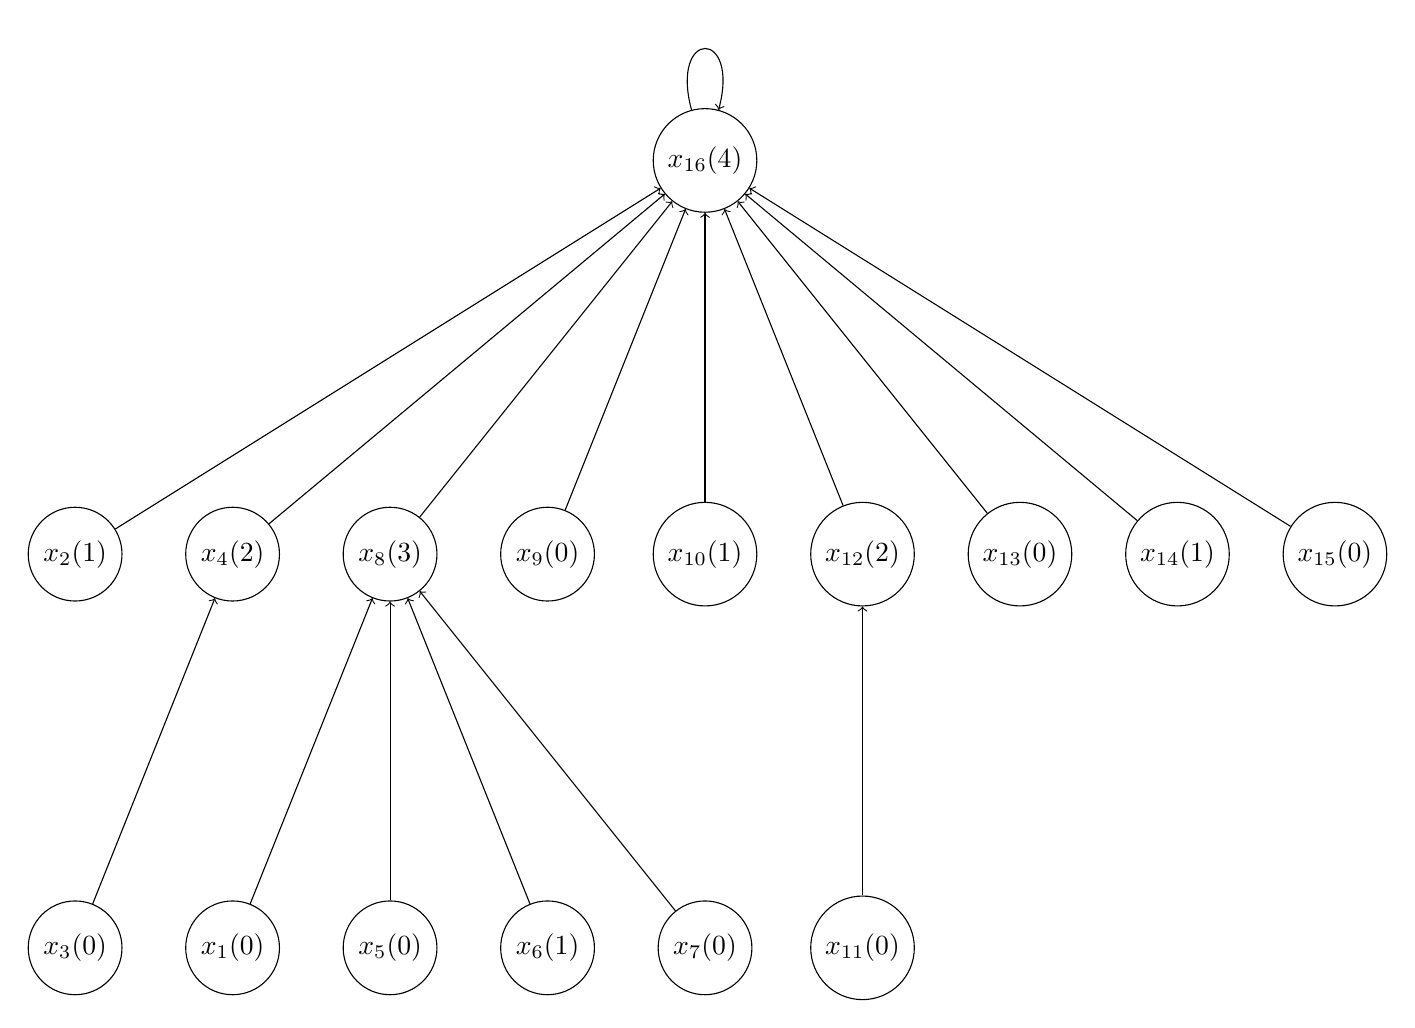
\begin{tikzpicture}
    \tikzset{vertex/.style = {shape=circle,draw,minimum size=1em}}
    \tikzset{edge/.style = {->,> = latex'}}
    \node[vertex] (x1) at (2,0) {$x_1 (0)$};
    \node[vertex] (x2) at (0,5) {$x_2 (1)$};
    \node[vertex] (x3) at (0,0) {$x_3 (0)$};
    \node[vertex] (x4) at (2,5) {$x_4 (2)$};
    \node[vertex] (x5) at (4,0) {$x_5 (0)$};
    \node[vertex] (x6) at (6,0) {$x_6 (1)$};
    \node[vertex] (x7) at (8,0) {$x_7 (0)$};
    \node[vertex] (x8) at (4,5) {$x_8 (3)$};
    \node[vertex] (x9) at (6,5) {$x_9 (0)$};
    \node[vertex] (x10) at (8,5) {$x_{10} (1)$};
    \node[vertex] (x11) at (10,0) {$x_{11} (0)$};
    \node[vertex] (x12) at (10,5) {$x_{12} (2)$};
    \node[vertex] (x13) at (12,5) {$x_{13} (0)$};
    \node[vertex] (x14) at (14,5) {$x_{14} (1)$};
    \node[vertex] (x15) at (16,5) {$x_{15} (0)$};
    \node[vertex] (x16) at (8,10) {$x_{16} (4)$};
    \draw[->] (x1) to (x8);
    \draw[->] (x2) to (x16);
    \draw[->] (x3) to (x4);
    \draw[->] (x4) to (x16);
    \draw[->] (x5) to (x8);
    \draw[->] (x6) to (x8);
    \draw[->] (x7) to (x8);
    \draw[->] (x8) to (x16);
    \draw[->] (x9) to (x16);
    \draw[->] (x10) to (x16);
    \draw[->] (x11) to (x12);
    \draw[->] (x12) to (x16);
    \draw[->] (x13) to (x16);
    \draw[->] (x14) to (x16);
    \draw[->] (x15) to (x16);
    \draw[->, loop above] (x16) to (x16);
\end{tikzpicture}

Hence $\proc{Find-Set}(x_2)$ and $\proc{Find-Set}(x_11)$
return a pointer points to $x_16$.

\subsection*{21.3-2}

\begin{minted}[xleftmargin=20pt,linenos]{cpp}
Node* FindSet(Node *x)
{
    Node *representative, *tmp;
    representative = x;
    while (representative != representative->p)
    {
        representative = representative->p;
    }
    while (x->p != representative)
    {
        tmp = x->p;
        x->p = representative;
        x = tmp;
    }
    return representative;
}
\end{minted}

\subsection*{21.3-3}

Note that we are proving that the upper bound $O(m \lg n)$ is tight (least upper bound),
instead of prove it is a tight bound $\Theta(m \lg n)$.
In order to prove it, we just need to find an example that takes $\Omega(m \lg n)$ time,
which is what the question is asking for.
We want our sequence to take as much as possible time.
WLOG, assume that $n = 2^k$ for some $k \in \NN$.
Consider the following sequence:
\begin{equation*}
\begin{split}
    \langle 
    & \proc{Make-Set}(x_1), \proc{Make-Set}(x_2), \cdots, \proc{Make-Set}(x_n), \\
    & \proc{Union}(x_1, x_2), \proc{Union}(x_3, x_4), \cdots, \proc{Union}(x_{n-1}, x_{n}), \\ 
    & \proc{Union}(x_1, x_3), \proc{Union}(x_5, x_7), \cdots, \proc{Union}(x_{n-3}, x_{n-1}), \\ 
    & \proc{Union}(x_1, x_5), \proc{Union}(x_9, x_13), \cdots, \proc{Union}(x_{n-7}, x_{n-3}), \\ 
    & \quad\quad\quad\quad\quad \vdots \\
    & \proc{Union}(x_1, x_{n / 2 + 1}), \\ 
    & \proc{Find-Set}(x_1) \cdots \quad\quad\quad \text{(until all $m$ operations are performed)} 
    \rangle
\end{split}
\end{equation*}
We performed $n$ $\proc{Make-Set}$, $(n-1)$ $\proc{Union}$, and $(m - 2n + 1)$ $\proc{Find-Set}$.
We observed we performed $n / 2$ $\proc{Union}(x_i, x_{i+1})$, $n / 4$ $\proc{Union}(x_i, x_{i+2})$,
$n / 8$ $\proc{Union}(x_i, x_{i+4})$, $\cdots$.
We conclude we performed $n / 2^j$ $\proc{Union}(x_i, x_{i+2^{j-1}})$ 
for all $j = \{ 1, 2, \cdots, \lg n \}$.
For each $j$, the height of each tree increases by $1$.
Hence after all $(n-1)$ $\proc{Union}$ operations,
the height of the tree (for the only set) is $\lg n$.
Note that $x_1$ is the deepest element in the tree.
Then, each of $\proc{Find-Set}(x_1)$ operation takes $\Theta(\lg n)$ time, 
and we perform $(m - 2n + 1)$ times $\proc{Find-Set}(x_1)$ operation.
Hence all of $\proc{Find-Set}(x_1)$ take $(m - 2n + 1)\Theta(\lg n) = \Theta(m \lg n)$ time.
We successfully find a sequence that takes $\Omega(m \lg n)$ time.

\subsection*{21.3-4}

We just need to modify $\proc{Link}$ procedure to maintain the data structure.

\begin{minted}[xleftmargin=20pt,linenos]{cpp}
void Link(Node *x, Node *y)
{
    Node *y_next;
    if (x->rank > y->rank)
    {
        y->p = x;
    }
    else
    {
        x->p = y;
        if (x->rank == y->rank)
            ++y->rank;
    }
    // maintain the circular list
    y_next = y->next;
    y->next = x->next;
    x->next = y_next;
}

std::list<Node*> PrintSet(Node *x)
{
    Node *node;
    std::list<Node*> result;
    result.push_back(x);
    for (node = x->next; node != x; node = node->next)
    {
        result.push_back(node);
    }
    return result;
}
\end{minted}

\subsection*{21.3-5}

Let $a_i$ be the number of nodes with depth greater than 0 
(i.e. non-root) in the forest after the $i$th operation.
Let $b_i$ be the number of nodes with depth greater than 1 
(i.e. non-root and non-child-of-root) in the forest after the $i$th operation.
Suppose that we start to perform $\proc{Find-Set}$ operations in the $k$th operation.
Let the potential function be
\begin{equation*}
    \Phi(D_i)
    \begin{cases}
        a_i & \text{if } i < k \text{ ,} \\
        b_i & \text{if } i \geq k \\
    \end{cases}
\end{equation*}
where $D_i$ is the disjoint forest after the $i$th operation.
Let $\Phi(D_0) = 0$.
Observed each of $\proc{Make-Set}$ and $\proc{Link}$ takes $O(1)$ time.
Denote $depth_i(x)$ as the depth of the node $x$ in the tree after the $i$th operation.
Then $\proc{Find-Set}(x)$ moves $\func{max}(0,depth_{i-1}(x) - 1)$ nodes 
to be the children of the root node.
Denote $c_i$ as the cost of the $i$th operation.
Then we assume
\begin{equation*}
    c_i = 
    \begin{cases}
        1 & \text{if $\proc{Make-Set}$ is performed in the $i$th operation,} \\
        1 & \text{if $\proc{Link}$ is performed in the $i$th operation,} \\
        \func{max}(1,depth_{i-1}(x)) & \text{if $\proc{Find-Set}(x)$ is performed in the $i$th operation} \\
    \end{cases}
\end{equation*}

\textbf{Case 1.}
$\proc{Make-Set}$ is performed in the $i$th operation.

Then $a_i = a_{i-1}$, so
\begin{equation*}
    \hat{c_i} = c_i + \Phi(D_i) - \Phi(D_{i-1})
    = 1 + 0 = 1
\end{equation*}

\textbf{Case 2.}
$\proc{Link}(x,y)$ is performed in the $i$th operation.

Note that $x$ and $y$ must be root nodes of different tree.
This operation make either $x$ or $y$ be a non-root node.
Then $a_i = a_{i-1} + 1$, so
\begin{equation*}
    \hat{c_i} = c_i + \Phi(D_i) - \Phi(D_{i-1})
    = 1 + 1 = 2
\end{equation*}

\textbf{Case 3.}
$\proc{Find-Set}(x)$ is performed in the $i$th operation.

Note that $b_i \leq a_i$ for all $i$.
If $i = k$, then 
\begin{equation*}
    \Phi(D_i) - \Phi(D_{i-1})
    = b_{i} - a_{i - 1}
    \leq b_{i} - b_{i - 1}
\end{equation*}
If $i > k$, then
\begin{equation*}
    \Phi(D_i) - \Phi(D_{i-1})
    = b_{i} - b_{i - 1}
\end{equation*}
Note that 
\begin{equation*}
    b_{i} - b_{i - 1} = - (\func{max}(1,depth_{i-1}(x)) - 1) = 1 - \func{max}(1,depth_{i-1}(x))
\end{equation*}
Hence 
\begin{equation*}
    \hat{c_i} = c_i + \Phi(D_i) - \Phi(D_{i-1})
    \leq c_i + b_{i} - b_{i - 1}
    = \func{max}(1,depth_{i-1}(x)) + (1 - \func{max}(1,depth_{i-1}(x)))
    = 1
\end{equation*}

We have shown that amortized of each operation is $O(1)$ 
with the path-compression heuristic,
no matter whether we use union by rank or not.
Hence the sequence takes $O(m)$ time 
with the path-compression heuristic,
no matter whether we use union by rank or not.

\section*{21.4}

\subsection*{21.4-1}

\begin{proof}
    We prove by induction on the number of operations.
    
    \textit{(Base)}
    Initially, there is no element in the disjoint sets,
    so it is trivial.

    \textit{(Induction)}
    Denote $D_i$ be the data structure after $i$th operation.
    Denote $p_i(x)$ be $x.p$ after $i$th operation.
    Denote $rank_i(x)$ be $x.rank$ after $i$th operation.
    Suppose that, for all $x \in D_{i - 1}$,
    \textcircled{1} $rank_{i-1}(x) < rank_{i-1}(p_{i-1}(x))$ if $x \neq p_{i-1}(x)$,
    \textcircled{2} $rank_{i-1}(x) = rank_{i-2}(x)$ if $x \neq p_{i-1}(x)$, and
    \textcircled{3} $rank_{i-1}(p_{i-1}(x)) \geq rank_{i-2}(p_{i-2}(x))$.
    
    \textbf{Case 1.}
    $\proc{Make-Set}(y)$ is performed in the $i$th operation.
    
    Then all structures of trees in $D_{i-1}$ remain same in $D_i$,
    and \textcircled{1}\textcircled{2}\textcircled{3} are vacuously true for $y$. 

    \textbf{Case 2.}
    $\proc{Find-Set}(y)$ is performed in the $i$th operation.

    Since no rank changes in $\proc{Find-Set}$, \textcircled{2} holds.
    Let $z$ be the root of the tree contains $y$.
    Let $A$ be the set contains all the nodes on the simple path 
    from $y$ to $z$ except $z$ in $D_{i-1}$.
    Let $w \in A$ be arbitrary choice.
    We have $w \neq p_{i-1}(w)$.
    By \textcircled{1}, since $p_i(w) = z$, we have 
    \begin{equation*}
        rank_{i-1}(w) < rank_{i-1}(p_{i-1}(w)) \leq rank_{i-1}(z) = rank_{i-1}(p_i(w))
    \end{equation*}
    Since no rank changes in $\proc{Find-Set}$, we have 
    $rank_i(w) < rank_i(p_i(w))$ and $rank_i(p_i(w)) \geq rank_{i-1}(p_{i-1}(w))$.
    For all elements not in $A$, their $p$ are not changed in the $i$th operation.
    Thus, we conclude \textcircled{1}\textcircled{3} holds.
     
    \textbf{Case 3.}
    $\proc{Union}(y,z)$ is performed in the $i$th operation.
    Let $f$ be the root of the tree contains $y$,
    and let $g$ be the root of the tree contains $z$.
    $\proc{Union}(y,z)$ is acutally perfroming the following sequence
    \begin{equation*}
        \langle \proc{Find-Set}(y), \proc{Find-Set}(z), \proc{Link}(f,g)
    \end{equation*}
    By case 2, we know IH holds after $\proc{Find-Set}$.
    Then we assume \textcircled{1}\textcircled{2}\textcircled{3} holds for $(i-1)$th operation
    and we are performing $\proc{Link}(f,g)$ in the $i$th operation.
    There are three subcases: $rank_{i-1}(f) > rank_{i-1}(g)$, $rank_{i-1}(f) < rank_{i-1}(g)$,
    and $rank_{i-1}(f) = rank_{i-1}(g)$; we notice the first two are similar, 
    so we ignore the first subcase.
    First, we suppose that $rank_{i-1}(f) < rank_{i-1}(g)$.
    Notice that $f$ is the only node that $p$ attribute is changed in the $i$th operation.
    We have $p_{i-1}(f) = f$ and $p_i(f) = g$.
    Then
    \begin{equation*}
        rank_{i-1}(p_{i-1}(f)) = rank_{i-1}(f) < rank_{i-1}(g) = rank_{i-1}(p_i(f))
    \end{equation*}
    Since no rank changes in this subcase, we have 
    $rank_{i}(f) < rank_{i}(p_i(f))$ and $rank_{i}(p_i(f)) \geq rank_{i-1}(p_{i-1}(f))$.
    Thus, we conclude \textcircled{1}\textcircled{2}\textcircled{3} holds.
    Now, we suppose that $rank_{i-1}(f) = rank_{i-1}(g)$.
    By the similar approach to the last subcase, we have
    \begin{equation*}
        rank_{i-1}(p_{i-1}(f)) = rank_{i-1}(f) = rank_{i-1}(g) = rank_{i-1}(p_i(f))
    \end{equation*}
    By line 5 of the procedure, we have $rank_{i}(g) = rank_{i-1}(g) + 1$,
    and ranks of all nodes except $g$ remain same in the $i$th operation.
    Then
    \begin{equation*}
        rank_{i-1}(p_{i-1}(f)) = rank_{i}(f) = rank_{i-1}(f) = rank_{i-1}(g) = rank_{i}(g) - 1 < rank_{i}(g) = rank_{i}(p_i(f))
    \end{equation*}
    Hence \textcircled{1}\textcircled{2}\textcircled{3} holds for $f$.
    Since $p_{i-1}(g) = p_i(g) = g$, we have
    \begin{equation*}
        rank_{i-1}(p_{i-1}(g)) = rank_{i-1}(g) = rank_{i}(g) - 1 < rank_{i}(g) = rank_{i}(p_i(g))
    \end{equation*}
    Hence \textcircled{1}\textcircled{2}\textcircled{3} holds for $g$ 
    (\textcircled{1}\textcircled{2} are vacuously true).
    For all nodes other than $f$ and $g$, rank and p attributes remain same in $i$th operation.
    Thus, we conclude \textcircled{1}\textcircled{2}\textcircled{3} holds.
\end{proof}

\subsection*{21.4-2}

\begin{lemma}
    If there exist a node has rank of $k$,
    then there exists at least $2^k$ nodes in the forest.
\end{lemma}

\begin{proof}
    \textit{(Base)}
    If there exist a node has rank of $0$, 
    there is at least one node in the forest.

    \textit{(Induction)}
    Suppose that the lemma is true for $k = h$ for some $h \geq 0$.
    Consider $k = h + 1$.
    If there exist a node has rank of $h + 1$,
    then, by line 4 of $\proc{Link}$, 
    there must were at least two node have rank of $h$ before.
    By the inductive hypothesis, 
    there exists at least $2 \cdot 2^k = 2^{k+1}$ nodes in the forest.
\end{proof}

\begin{claim}
    In an $n$ disjoint sets using union by rank and path compression heuristic, 
    every node has rank at most $\lfloor \lg n \rfloor$.
\end{claim}

\begin{proof}
    Suppose that their exist a node has rank of $\lfloor \lg n \rfloor + 1$,
    for the purpose of contradiction.
    By the lemma, there exists at least $2^{\lfloor \lg n \rfloor + 1}$ nodes
    in the forest.
    \begin{equation*}
        2^{\lfloor \lg n \rfloor + 1} > 2^{\lg n} = n
    \end{equation*}
    Contradiction.
\end{proof}

\subsection*{21.4-3}

We need $\lceil \lg (k + 1) \rceil$ bits to store value $k$.
Hence $\lceil \lg (\lfloor \lg n \rfloor + 1) \rceil$ bits
are necesary to store $x.rank$. 

\subsection*{21.4-4}

\begin{proof}
    Taking advantage of Lemma 21.7, we convert the sequence into 
    a sequence of $m$ $\proc{Make-Set}$, $\proc{Link}$, and $\proc{Find-Set}$.
    Without path compression, 
    rank of each node is exactly the height of the node.
    Observed $\proc{Make-Set}$ and $\proc{Link}$ take $O(1)$ time,
    and $\proc{Find-Set}(x)$ takes $O(x.rank)$ time.
    Hence the sequence run in $O(m \lg n)$ time.
\end{proof}

\subsection*{21.4-5}

No.
Consider $x.rank = 1$, $x.p.rank = 7$, and $x.p.p.rank = 8$.
Clearly, $x.rank > 0$ and $x.p$ is not a root.
Since 
\begin{equation*}
    A_2(x.rank) = A_2(1) = 7
\end{equation*}
and
\begin{equation*}
    A_3(x.rank) = A_3(1) = 2047 \quad,
\end{equation*}
we have
\begin{equation*}
    A_2(x.rank) \leq x.p.rank < A_3(x.rank) \quad,
\end{equation*}
so
\begin{equation*}
    \func{level}(x) = 2 \quad.
\end{equation*}
Since
\begin{equation*}
    A_0(x.p.rank) = A_0(7) = 8
\end{equation*}
and
\begin{equation*}
    A_1(x.p.rank) = A_1(7) = 15 \quad,
\end{equation*}
we have
\begin{equation*}
    A_0(x.p.rank) \leq x.p.p.rank < A_1(x.p.rank) \quad,
\end{equation*}
so
\begin{equation*}
    \func{level}(x.p) = 0 \quad.
\end{equation*}
Therefore,
\begin{equation*}
    \func{level}(x) > \func{level}(x.p) \quad.
\end{equation*}

\subsection*{21.4-6}

Since $A_3(1) = 2047$, $\alpha'(n) \leq 3$ implies
\begin{equation*}
    A_3 = 2047 \geq \lg (n + 1) \quad.
\end{equation*}
Then 
\begin{equation*}
    n \leq 2^{2047} - 1 = \frac{2^{2048}}{2} - 1 
    = \frac{(2^4)^{512}}{2} - 1 = 16^{511} - 1 \gg 10^{80} \quad.
\end{equation*}

Replace all $\alpha(n)$ with $\alpha'(n)$ in the argument.
The only modification we need to make is at the bound (21.1).
We claim that
\begin{equation*}
    0 \leq \func{level}(x) < \alpha'(n) \quad.
\end{equation*}
We need to modify the argument to prove $\func{level}(x) < \alpha'(n)$.
\begin{equation*}
\begin{split}
    A_{\alpha'(n)}(x.rank) & \geq A_{\alpha'(n)}(1)
    \text{\indent(bacause $A_k(j)$ is strictly increasing)} \\
    & \geq \lg (n + 1) 
    \text{\indent(by the definition of $\alpha'(n)$)} \\
    & > \lfloor \lg(n) \rfloor \\
    & \geq x.p.rank
    \text{\indent(by exercise 21.4-2)} \\
\end{split}
\end{equation*}

\section*{Chapter 21 Problems}

\subsection*{21-1}

\subsubsection*{(a)}

$[ 4, 3, 2, 6, 8, 1 ]$

\subsubsection*{(b)}

\begin{proof}
    \textit{(Base)}
    Let $j \in \{ 1, 2, \cdots, m \}$,
    and let $t \in K_j$.
    Suppose that $extracted[k] = t$ 
    for some $k \in \{ 1, 2, \cdots, j - 1 \}$,
    for the purpose of contradiction.
    Then $extracted[k]$ is extracting the value from $K_j$
    where $j > k$.
    Contradiction.

    \textit{(Induction)}
    Assume the value is removed from the set after we extract it.
    Suppose that \textcircled{1}
    \begin{equation*}
        \forall j \in \{ 1, 2, \cdots, m \},
        \forall t \in K_j, 
        extracted[k] = t
        \text{ for some } k \in \{ j, j + 1, \cdots, m \}
        \text{ or $t$ will not be extracted }
        \quad,
    \end{equation*}
    and suppose that \textcircled{2} 
    any values in $\{ 1, 2, \cdots, i - 1 \}$ 
    have been extracted correctly (hence these values are removed from  
    $\bigcup\limits_{j \in \{ 1, 2, \cdots, m \}} K_j$).
    Then at this time, $i$ is the smallest value
    that is not in the $extracted$ array.
    Now, we determine $j$ such that $i \in K_j$.
    By the hypothesis \textcircled{1}, we know that $extracted[k] = i$
    for some $k \in \{ j, j + 1, \cdots, m \}$ 
    or $i$ will not be extracted.
    Since $extracted[j]$ extracted value
    early than $extracted[j + 1], extracted[j + 2], \cdots, extracted[m]$,
    we know $extracted[j]$ extracted the smallest possible value $i$, 
    and this value is what $\proc{Off-Line-Minimum}$
    will choose, so we have shown that $i$ is extracted correctly.
    Hence \textcircled{2} holds.
    Let $l$ be the smallest value greater than $j$ 
    for which set $K_l$ exists (i.e. $extracted[l]$ was empty).
    Let $A = K_j$ for facilitating our analysis to $K_j$ after destroying $K_j$.
    Now, we performed $K_l = K_k \cup K_l$ and destroyed $K_j$,
    we claim the hypothesis \textcircled{1} holds.
    By the way we choosed $l$, we knew 
    $extract[j], extracted[j + 1], \cdots, extracted[l - 1]$
    were nonempty, so for all $t \in A$,
    $extracted[k] = t$ only if $k \neq j, j + 1, \cdots, l - 1$.
    Then for all $t \in A$, 
    $extracted[k] = t$ for some $k \in \{ j, j + 1, \cdots, m \}$
    or $t$ will not be extracted.
    Hence \textcircled{1} holds.
\end{proof}

\subsubsection*{(c)}

\begin{minted}[xleftmargin=20pt,linenos]{cpp}
struct Node
{
    int p;
    int rank;
    // set info:
    int subsequence_index_lower;// only root
    int subsequence_index_upper;// only root
    int prev;// only root
    int next;// only root
};

int FindSet(std::vector<Node>& forest, int x)
{
    if (forest[x].p != x)
        forest[x].p = FindSet(forest, forest[x].p);
    return forest[x].p;
}

// keep y's set info
void Link(std::vector<Node>& forest, int x, int y)
{
    forest[forest[x].prev].next = forest[x].next;
    forest[forest[x].next].prev = forest[x].prev;
    if (forest[x].rank > forest[y].rank)
    {
        forest[y].p = x;
        forest[x].subsequence_index_lower = forest[y].subsequence_index_lower;
        forest[x].subsequence_index_upper = forest[y].subsequence_index_upper;
        forest[x].prev = forest[y].prev;
        forest[x].next = forest[y].next;
        forest[forest[x].prev].next = x;
        forest[forest[x].next].prev = x;
    }
    else
    {
        forest[x].p = y;
        if (forest[x].rank == forest[y].rank)
            ++forest[y].rank;
    }
}

void Union(std::vector<Node>& forest, int x, int y)
{
    return Link(forest, FindSet(forest, x), FindSet(forest, y));
}

// operations: E represents by -1
// n: domain size
std::vector<int> OffLineMinimum(const std::vector<int>& operations, int n)
{
    int i, j, m, root, last_root;
    std::vector<Node> forest(n + 1);// index start by 1
    // init disjoin-set forest
    for (i = 1; i <= n; ++i)
    {
        forest[i].p = i;
        forest[i].rank = 0;
    }
    // init subsequence
    m = 1;
    root = 0;
    last_root = 0;
    for (i = 0; i < operations.size(); ++i)
    {
        if (operations[i] < 0)
        {
            // extract
            forest[root].subsequence_index_upper = m;
            ++m;
            last_root = root;
        }
        else if (last_root == root)
        {
            // first insert in the subsequence
            root = operations[i];
            forest[root].subsequence_index_lower = m;
            forest[root].prev = last_root;
            forest[last_root].next = root;
        }
        else
        {
            // non-first insert in the subsequence
            forest[operations[i]].p = root;
            forest[root].rank = 1;
        }
    }
    m = forest[last_root].subsequence_index_upper;
    forest[last_root].next = 0;// for situation of that the last operation is extract
    forest[0].subsequence_index_lower = m + 1;
    // compute extracted array
    std::vector<int> extracted(m);
    for (i = 1; i <= n; ++i)
    {
        root = FindSet(forest, i);
        j = forest[root].subsequence_index_lower;
        if (j <= m)
        {
            extracted[j - 1] = i;
            if (forest[root].subsequence_index_lower < forest[root].subsequence_index_upper)
                ++forest[root].subsequence_index_lower;
            else
                Union(forest, root, forest[root].next);
        }
    }
    return extracted;
}
\end{minted}
    
In the worst-case, the running time is $O(n \alpha(n))$.

\subsection*{21-2}

\subsubsection*{(a)}

\begin{proof}
    Suppose that we performed $n$ times $\proc{Make-Tree}$.
    To maximize the depth we performed $n - 1$ times $\proc{Graft}$
    to form a tree where the depth of leaf is $n - 1$ 
    (the tree become a linked list contains all $n$ nodes).
    Then we performed $m - 2n + 1$ $\proc{Find-Depth}$ on the leaf.
    Each of $\proc{Make-Tree}$ and $\proc{Graft}$ takes $\Theta(1)$ time,
    and each of $\proc{Find-Depth}$ takes $\Theta(n)$ time.
    Hence the sequence takes
    \begin{equation*}
        \underbrace{n \cdot \Theta(1)}_{\proc{Make-Tree}}
        + \underbrace{(n - 1) \cdot \Theta(1)}_{\proc{Graft}}
        + \underbrace{(m - 2n + 1) \cdot \Theta(n)}_{\proc{Find-Depth}}
        = O(mn)
    \end{equation*}
    time in total.
    Consider $n = \frac{m}{3}$.
    In this case, the sequence takes $\Theta(m^2)$ time.
\end{proof}

\subsubsection*{(b)}

\begin{minted}[xleftmargin=20pt,linenos]{cpp}
void MakeTree(Node *x)
{
    x->p = x;
    x->rank = 0;
    x->d = 0;
}
\end{minted}

\subsubsection*{(c)}

\begin{minted}[xleftmargin=20pt,linenos]{cpp}
// after the function return, v->p is the root of the tree in the disjoint sets
void Compression(Node *v)
{
    if (v->p != v->p->p)
    {
        Compression(v->p);
        v->d += v->p->d;
        v->p = v->p->p;
    }
}

// after the function return, v->p is the root of the tree in the disjoint sets
int FindDepth(Node *v)
{
    Compression(v);
    return (v == v->p) ? v->d : (v->d + v->p->d);
}
\end{minted}

\subsubsection*{(d)}

\begin{minted}[xleftmargin=20pt,linenos]{cpp}
void Graft(Node *r, Node *v)
{
    Node *r_set, *v_set;
    Compression(r);
    // r_set is the root node of the disjoint set contains r
    r_set = r->p;
    // add depths of all nodes in the tree contains node r by the depth of node v
    // correctness: disjoint set contains r is 
    //              exactly the set contains all elements in the tree contains r  
    r_set->d += (FindDepth(v) + 1);
    // v_set is the root node of the disjoint set contains v
    v_set = v->p;
    if (r_set->rank > v_set->rank)
    {
        v_set->p = r_set;
        // since r_set becomes parent of v_set in the disjoint set,
        // we need to subtract pseudodistance of v_set by that of r_set
        v_set->d -= r_set->d;
    }
    else
    {
        r_set->p = v_set;
        // since v_set becomes parent of r_set in the disjoint set,
        // we need to subtract pseudodistance of r_set by that of v_set
        r_set->d -= v_set->d;
        if (r_set->rank == v_set->rank)
            ++v_set->rank;
    }
}
\end{minted}

\subsubsection*{(e)}

$\Theta(m \alpha(n))$ where $n$ is the number of nodes in the forest.

\subsection*{21-3}

\subsubsection*{(a)}

\begin{proof}
    $\proc{LCA}$ is actually doing a postorder tree walk
    (the walk executes lines 8 - 10 for the root after doing so for the subtrees).
    Then each pair in $P$ will be processed twice at line 8, 9.
    Note that the procedure blanken the node after the node is visted.
    Let $\{ u, v \}$ be an arbitrary choice.
    WLOG, assume $u$ is visited before $v$.
    At the time of $u$ is being visiting, $v$ has not been visited,
    so $v.color \neq BLACK$, 
    and line 10 does not execute for the pair $\{ u, v \}$, therefore.
    At the time of $v$ is being visiting, $v$ has already been visited,
    so $v.color == BLACK$, 
    and line 10 executes for the pair $\{ u, v \}$, therefore.
    Thus, line 10 executes exactly once for each pair $\{ u, v \} \in P$ .
\end{proof}

\subsubsection*{(b)}

\begin{proof}
    Denote $height(u)$ as the height of the node $u$ in $T$,
    and denote $depth(u)$ as the depth of the node $u$ in $T$.

    \textit{(Base)}
    Let $u \in T$ where $height(u) = 0$.
    Then $u$ do not have any descendant.
    Suppose that at the time of the call $\proc{LCA}(u)$, the number of sets is $depth(u)$.
    Then at the time of $\proc{LCA}(u)$ return, the number of sets is $depth(u) + 1$,
    where the new set is from $\func{Make-Set}(u)$ at line 1.
    Thus the inductive hypothesis (see below) holds for all $u \in T$ where $height(u) = 0$.

    \textit{(Induction)}
    Inductive hypothesis: for all $u \in T$ where $height(u) \leq k$, 
    if at the time of the call $\proc{LCA}(u)$, the number of sets is $depth(u)$,
    then at the time of the call $\proc{LCA}(v)$ where $v$ is a descendant of $u$, 
    the number of sets is $depth(v)$, 
    and at the time of $\proc{LCA}(u)$ return, the number of sets is $depth(u) + 1$.

    Let $u \in T$ where $height(u) = k + 1$.
    Suppose that at the time of the call $\proc{LCA}(u)$, the number of sets is $depth(u)$.
    Then at the time after line 2 of $\proc{LCA}(u)$ is executed, 
    the number of sets is $depth(u) + 1$.
    We claim that after the $\For$ loop (line 3 - 6),
    the number of sets is $depth(u) + 1$.
    At line 4, we call $\proc{LCA}(v)$ where $v$ is a child of $u$.
    Then $height(v) < height(u)$, so $height(v) \leq k$.
    And the number of sets is $depth(u) + 1 = depth(v)$.
    By the inductive hypothesis, at the time of $\proc{LCA}(v)$ return, 
    the number of sets is $depth(v) + 1 = (depth(u) + 1) + 1 = depth(u) + 2$.
    And we have at the time of the call $\proc{LCA}(w)$ where $w$ is a descendant of $v$, 
    the number of sets is $depth(w)$.
    At line 5, we perform $\proc{Union}(x,y)$, so at this time, 
    the number of sets is $depth(u) + 2 - 1 = depth(u) + 1$.
    Thus, after the $\For$ loop,
    the number of sets is $depth(u) + 1$,
    and the number of sets is same at the time of $\proc{LCA}(u)$ return.
    Hence the inductive hypothesis holds for all $u \in T$ where $height(u) \leq k + 1$.

    \textit{(Conclusion)}
    By mathmatical induction, 
    since at the time of the call $\proc{LCA}(T.root)$, the number of sets is $depth(T.root) = 0$,
    and all nodes in $T$ is a descendant of $T.root$,
    we conclude at the time of the call $\proc{LCA}(u)$, the number of sets is $depth(u)$.
\end{proof}

\subsubsection*{(c)}

Denote $T_u$ as the subtree rooted at $u$.

\begin{lemma}
    Suppose that the program is currently running in $\proc{LCA}(a)$
    (i.e. the top of the call stack is $\proc{LCA}(a)$) at the end of the line 6.
    Let $B$ be the set contains all black color children of $a$.
    Let $A = a \cup \bigcup\limits_{b \in B} T_b$.
    Then the disjoint set of node $a$ is exactly set $A$  
    and $\proc{Find-Set}(a).ancestor = a$.
\end{lemma}

\begin{proof}
    \textit{(Base)}
    Let $a \in T$ where $height(a) = 0$.
    Then $a$ does not have any children.
    Thus, at the end of line 6 
    (consider the start of line 7 here) of $\proc{LCA}(a)$, 
    the disjoint set of node $a$ only contains $a$,
    and $\proc{Find-Set}(a).ancestor = a$ by line 2.

    \textit{(Induction)}
    Suppose that the lemma is true for all $a$ where $height(a) \leq k$.
    Let $a \in T$ where $height(a) = k + 1$.
    Let $B$ be the set contains all black color children of $a$.
    Then for all $b \in B$, $height(b) \leq k$.
    Since $b.color$ is black, the colors of all children of $b$ are black.
    By the hypothesis, all elements in $T_b$ are in a same disjoint set.
    At line 5 - 6, we union all elements in $T_b$ with $a$.
    Thus, the disjoint set of node $a$ is $a \cup \bigcup\limits_{b \in B} T_b$.
    We have $\proc{Find-Set}(a).ancestor = a$ by line 6 immediately.
\end{proof}

\begin{claim}
    Suppose the program is currently running in $\proc{LCA}(u)$
    (i.e. the top of the call stack is $\proc{LCA}(u)$).
    Then for all $v \in T$ where $u \neq v$, if $v.color$ is BLACK,
    then $\proc{Find-Set}(v).ancestor$ is the least common ancestor of $u$ and $v$.
\end{claim}

Note that it is impossible to have $v$ to be a proper ancestor of $u$.

\begin{proof}
    Let $u, v \in T$ where $u \neq v$, and let $a$ be the least common ancestor of $u$ and $v$.

    Suppose that the program is currently running in $\proc{LCA}(a)$,
    $u$ has not been visited, and $v$ has been visited.
    Then $u.color$ is WHITE, and $v.color$ is BLACK.
    Let $b \in T$ such that $b$ is a child of $a$ and $v$ is a descendant of $b$ 
    (i.e. $v \in T_b$). 
    Since the program is currently running in $\proc{LCA}(a)$,
    $b.color$ must be BLACK also.
    By the lemma, we have $\proc{Find-Set}(v) = \proc{Find-Set}(a)$
    and $\proc{Find-Set}(v).ancestor = \proc{Find-Set}(a).ancestor = a$. 

    Suppose that the program keeps running and is currently running in $\proc{LCA}(u)$.
    When the top of the call stack is not $\proc{LCA}(u)$ 
    and the call stack still contains $\proc{LCA}(u)$,
    the disjoint set contains $a$ must remains same.
    Thus, $\proc{Find-Set}(v).ancestor$ and $\proc{Find-Set}(a).ancestor$ still equal to $a$.
\end{proof}

\subsubsection*{(d)}

\begin{tabular}{c|c|c}
    operation & location & times \\
    \hline
    $\proc{Make-Set}$ & line 1 & $|T|$ \\
    $\proc{Find-Set}$ & line 2 & $|T|$ \\
    $\proc{Union}$ & line 5 & $|T| - 1$ \\
    $\proc{Find-Set}$ & line 6 & $|T| - 1$ \\
    $\proc{Find-Set}$ & line 10 & $|P|$ (by part (a)) \\
\end{tabular}

Hence $\proc{LCA}$ takes $O((|T| + |P|) \alpha(|T|))$.
Note that we can bound $|P|$ from above:
\begin{equation*}
    |P| \leq \binom{|T|}{2} = \Theta(|T|^2)
\end{equation*}
Then we can say that $\proc{LCA}$ takes $O(|T|^2 \alpha(|T|))$ also.

% \centerline{\textbf{Updating...}}

\end{document}